\chapter{Capstone: a transverse-field asymmetry measurement}
\label{ch:capstone}

\begin{willdo}
\begin{itemize}
  \item Assemble geometry, field, physics, beam and output into one simulation.
  \item Reproduce muon-spin precession in a transverse magnetic field.
  \item Build the asymmetry signal and fit a precession frequency.
  \item Recover the field you set from the frequency you measured.
\end{itemize}
\end{willdo}

Everything so far has been groundwork. Here we run a complete, if idealised, transverse-field muon spin rotation experiment: muons stop in a sample sitting in a magnetic field perpendicular to their spin, their spins precess, and the decay positrons are counted in two opposing detectors. The normalised difference of those counts oscillates at the Larmor frequency --- and from it we recover the field.

\section{The physics in one paragraph}
A muon spin in a magnetic field \(B\) precesses at the Larmor frequency \(f=(\gamma_\mu/2\pi)\,B\), with \(\gamma_\mu/2\pi\approx\SI{135.54}{MHz/T}\). The decay positron is emitted preferentially along the muon spin at the instant of decay. If the spin starts along the beam axis (\(z\)) and the field points along \(x\), the spin rotates in the \(y\)--\(z\) plane, so its \(y\)-component swings as \(\sin(2\pi f t)\). Two counters facing each other along \(\pm y\) therefore see their positron rates rise and fall in antiphase. The asymmetry
\[
A(t)=\frac{N_\mathrm{D}(t)-N_\mathrm{U}(t)}{N_\mathrm{D}(t)+N_\mathrm{U}(t)}
\]
cancels the exponential decay common to both counters and leaves a clean oscillation.

\begin{center}
\begin{tikzpicture}[font=\sffamily\scriptsize]
  \fill[cyanbg] (-3.2,1.55) rectangle (3.2,1.85);
  \draw[cyan] (-3.2,1.55) rectangle (3.2,1.85);
  \node[text=navy,above] at (0,1.85) {counter U at \(+y\) \quad (\texttt{CounterU}, \texttt{det\_ID 11})};
  \fill[cyanbg] (-3.2,-1.85) rectangle (3.2,-1.55);
  \draw[cyan] (-3.2,-1.85) rectangle (3.2,-1.55);
  \node[text=navy,below] at (0,-1.85) {counter D at \(-y\) \quad (\texttt{CounterD}, \texttt{det\_ID 1})};
  \fill[eblue!25] (-0.15,-0.6) rectangle (0.15,0.6);
  \draw[eblue] (-0.15,-0.6) rectangle (0.15,0.6);
  \node[text=navy,anchor=west] at (0.95,-1.1) {Cu \texttt{Target} (ID 5)};
  \draw[arr] (-4.6,0) -- (-0.2,0) node[pos=0.35,above,text=navy]{\(\mu^+\) beam along \(+z\)};
  \draw[-{Stealth[length=2mm]},navy,line width=0.9pt] (0,0) -- (-0.75,0) node[pos=1,below=3pt,text=navy]{spin};
  \draw[-{Stealth[length=2mm]},muted,dashed] (0.75,0) arc (0:300:0.75 and 0.75);
  \node[text=muted,anchor=west] at (0.95,0.55) {spin precesses in the \(y\)--\(z\) plane};
  \node[circle,draw=pitred,inner sep=1.6pt] (b) at (3.6,0) {}; \fill[pitred] (b) circle (0.7pt);
  \node[text=pitred,anchor=west] at (3.8,0) {\(\vec B\) along \(+x\) (out of page)};
  \draw[->,muted] (-4.6,-1.3) -- (-4.1,-1.3) node[right]{\(z\)};
  \draw[->,muted] (-4.6,-1.3) -- (-4.6,-0.8) node[above]{\(y\)};
\end{tikzpicture}
\end{center}

\section{The macro}
The geometry is a copper sample named \code{Target} and two scintillator plates, plus a uniform transverse field over the whole world and the standard physics block. The sample's name switches on the \code{muTarget...} branches, and the run keeps only muons that decayed inside it. The macro ships as \code{run/tf_musr.mac}:

\lstinputlisting[style=mac,caption={\texttt{tf\_musr.mac} --- a complete transverse-field experiment},label=lst:tf]{../run/tf_musr.mac}

\begin{lstlisting}[style=sh,caption={Run it (about 1.5 minutes on one core)}]
cd build/run
mkdir -p data
../musrSim tf_musr.mac        # -> data/musrSim_jp000_tf.root (suffix from SetOutputFileName)
\end{lstlisting}

The log confirms the field just before the first event: \code{Field at (0.00, 0.00, 0.00) mm is: B = (0.01, 0, 0) T}.

\begin{physics}
Surface muons at \SI{29.8}{MeV/c} stop within a fraction of a millimetre, so nearly all of them come to rest inside the \SI{6}{mm}-thick copper sample and decay there. The line \code{storeOnlyEventsWithMuonsDecayedInDetID 5} discards the few that stop elsewhere, so the analysis sees a clean sample-stopped population regardless of the exact stopping profile. Copper is also a good choice physically: muons in a non-magnetic metal do not form muonium and keep their full polarisation.
\end{physics}

\section{The analysis}
Load the tree, keep sample-stopped muons, and split the decay times by which counter caught the positron. Events in which \emph{both} counters fired are ambiguous and dropped. The exponential lifetime divides out of the asymmetry, leaving the precession.

\lstinputlisting[style=py,caption={\texttt{doc/scripts/asymmetry.py} --- from ROOT file to Larmor frequency},label=lst:asym]{scripts/asymmetry.py}

\section{What you should see}
In our reference run, 26\,224 positrons were counted in U and 25\,956 in D. The fit gives
\[
f = \SI{1.3530(20)}{MHz}\quad\Rightarrow\quad B = \frac{f}{\gamma_\mu/2\pi} = \SI{9.983(15)}{mT},
\]
within about one standard deviation of the \SI{10.000}{mT} we set --- a full round trip from a number in a macro to a field recovered from simulated positron counts (Figure~\ref{fig:asym}). The amplitude, \(A_0 = 0.266(9)\), sits below the maximum muon-decay asymmetry of \(1/3\) (averaged over all positron energies) because each counter accepts positrons over a wide range of angles.

\begin{figure}[h]
\centering
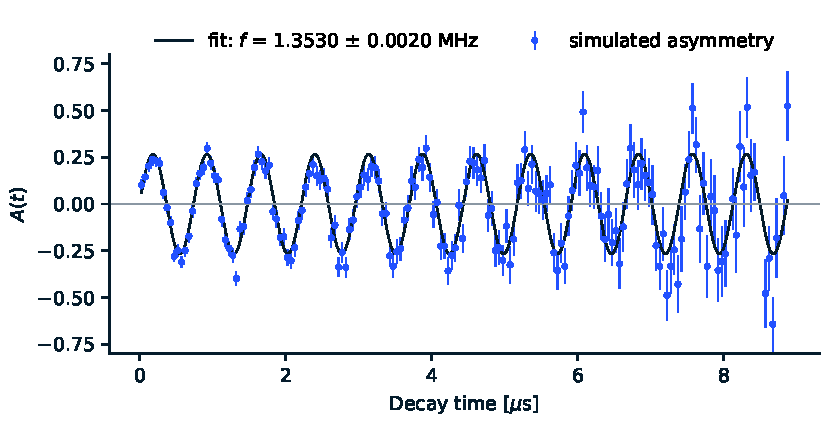
\includegraphics[width=0.86\textwidth]{figures/asymmetry.pdf}
\caption{Simulated positron asymmetry \(A(t)\) from \texttt{tf\_musr.mac} with the damped-sine fit. Error bars grow at late times as the surviving muons run out.}
\label{fig:asym}
\end{figure}

\begin{keypoint}
This closes the loop of the whole book. Geometry (Chapter~\ref{ch:geometry}) placed the counters; the physics block (Chapter~\ref{ch:macro}) let the muons stop and the positrons deposit energy; the field (Chapter~\ref{ch:fields}) drove the precession; the beam and spin (Chapter~\ref{ch:beam}) set the initial condition; the ROOT tree (Chapter~\ref{ch:output}) recorded \code{det_ID} and \code{muDecayTime}; and Python (Chapter~\ref{ch:python}) turned them into a number with a physical meaning.
\end{keypoint}

\begin{tip}
Turn this into a study. Scan the field by editing the one \code{0.01} in the macro, run each value (give each run its own suffix on the command line), and plot fitted frequency against set field --- it should be a straight line of slope \(\gamma_\mu/2\pi\). For a mapped field, the \code{<final> <nSteps>} ramp of Chapter~\ref{ch:fields} scans the field within a single run. Either is a genuine, if small, piece of \muSR\ physics.
\end{tip}

\begin{recap}
\begin{itemize}
  \item A complete experiment is a sample, two counters, a transverse field, the physics block and a polarised beam.
  \item The asymmetry \((N_\mathrm{D}-N_\mathrm{U})/(N_\mathrm{D}+N_\mathrm{U})\) cancels the lifetime and exposes the precession.
  \item Fitting the oscillation recovers the field you set, via \(f=(\gamma_\mu/2\pi)B\): \SI{9.983(15)}{mT} for \SI{10}{mT} set.
  \item Every skill from Chapters~\ref{ch:macro}--\ref{ch:fields} appears here as one part of a single physics result.
\end{itemize}
\end{recap}
\nextchap{troubleshooting, and reading the source}
